\documentclass[border=5pt]{standalone}
\usepackage{tikz}
\usetikzlibrary{shapes,arrows,positioning,fit,backgrounds,calc}

\begin{document}

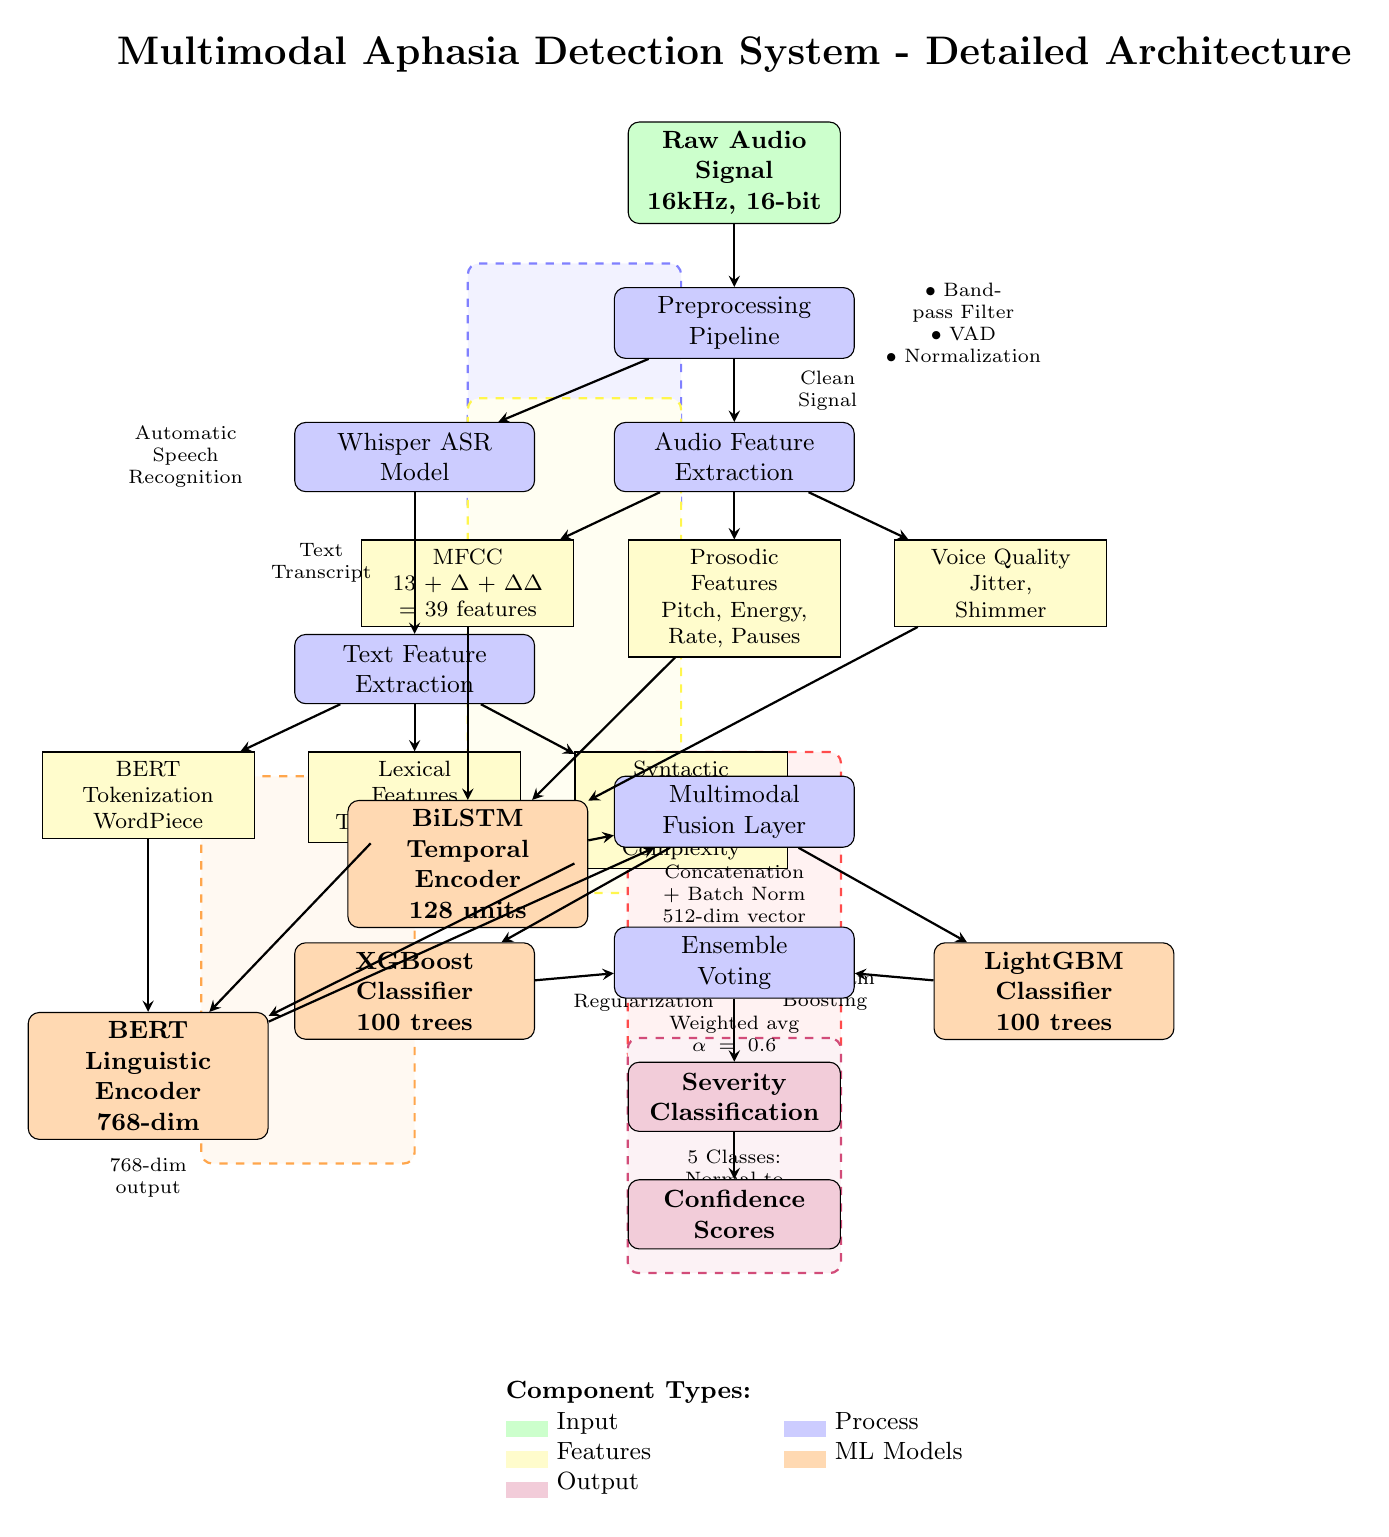
\begin{tikzpicture}[
    % Define styles
    input/.style={rectangle, draw, fill=green!20, text width=7em, text centered, rounded corners, minimum height=2.5em, font=\small\bfseries},
    process/.style={rectangle, draw, fill=blue!20, text width=8em, text centered, rounded corners, minimum height=2.5em, font=\small},
    feature/.style={rectangle, draw, fill=yellow!20, text width=7em, text centered, minimum height=2em, font=\footnotesize},
    model/.style={rectangle, draw, fill=orange!30, text width=8em, text centered, rounded corners, minimum height=3em, font=\small\bfseries},
    decision/.style={diamond, draw, fill=red!20, text width=5em, text centered, font=\footnotesize},
    output/.style={rectangle, draw, fill=purple!20, text width=7em, text centered, rounded corners, minimum height=2.5em, font=\small\bfseries},
    arrow/.style={thick,->,>=stealth},
    label/.style={font=\scriptsize, text width=6em, align=center}
]

% Input Layer
\node [input] (audio) {Raw Audio Signal\\16kHz, 16-bit};

% Preprocessing
\node [process, below=0.8cm of audio] (preprocess) {Preprocessing\\Pipeline};
\node [label, right=0.2cm of preprocess] {$\bullet$ Bandpass Filter\\$\bullet$ VAD\\$\bullet$ Normalization};

% ASR Module
\node [process, below left=0.8cm and 1cm of preprocess] (asr) {Whisper ASR\\Model};
\node [label, left=0.2cm of asr] {Automatic\\Speech\\Recognition};

% Feature Extraction - Audio Stream
\node [process, below=0.8cm of preprocess] (audio_feat) {Audio Feature\\Extraction};

\node [feature, below left=0.6cm and 0.5cm of audio_feat] (mfcc) {MFCC\\13 + $\Delta$ + $\Delta\Delta$\\= 39 features};
\node [feature, below=0.6cm of audio_feat] (prosody) {Prosodic\\Features\\Pitch, Energy,\\Rate, Pauses};
\node [feature, below right=0.6cm and 0.5cm of audio_feat] (voice) {Voice Quality\\Jitter,\\Shimmer};

% Feature Extraction - Text Stream
\node [process, below=1.8cm of asr] (text_feat) {Text Feature\\Extraction};

\node [feature, below left=0.6cm and 0.5cm of text_feat] (bert_tok) {BERT\\Tokenization\\WordPiece};
\node [feature, below=0.6cm of text_feat] (lexical) {Lexical\\Features\\TTR, Diversity};
\node [feature, below right=0.6cm and 0.5cm of text_feat] (syntax) {Syntactic\\Features\\FK Grade,\\Complexity};

% Deep Learning Models
\node [model, below=2.2cm of mfcc] (lstm) {BiLSTM\\Temporal\\Encoder\\128 units};
\node [model, below=2.2cm of bert_tok] (bert) {BERT\\Linguistic\\Encoder\\768-dim};

% Feature Dimensions
\node [label, below=0.1cm of lstm] {256-dim\\output};
\node [label, below=0.1cm of bert] {768-dim\\output};

% Fusion Layer
\node [process, below=1.5cm of prosody] (fusion) {Multimodal\\Fusion Layer};
\node [label, below=0.1cm of fusion] {Concatenation\\+ Batch Norm\\512-dim vector};

% Ensemble Classifiers
\node [model, below left=1.2cm and 1cm of fusion] (xgb) {XGBoost\\Classifier\\100 trees};
\node [model, below right=1.2cm and 1cm of fusion] (lgbm) {LightGBM\\Classifier\\100 trees};

\node [label, right=0.2cm of xgb] {L1/L2\\Regularization};
\node [label, left=0.2cm of lgbm] {Histogram\\Boosting};

% Ensemble Fusion
\node [process, below=1cm of fusion] (ensemble) {Ensemble\\Voting};
\node [label, below=0.1cm of ensemble] {Weighted avg\\$\alpha=0.6$};

% Output
\node [output, below=0.8cm of ensemble] (severity) {Severity\\Classification};
\node [label, below=0.1cm of severity] {5 Classes:\\Normal to\\Very Severe};

\node [output, below=0.6cm of severity] (confidence) {Confidence\\Scores};

% Draw arrows with labels
\draw [arrow] (audio) -- (preprocess);
\draw [arrow] (preprocess) -- node[right, label] {Clean\\Signal} (audio_feat);
\draw [arrow] (preprocess) -- (asr);
\draw [arrow] (asr) -- node[left, label] {Text\\Transcript} (text_feat);

% Audio features
\draw [arrow] (audio_feat) -- (mfcc);
\draw [arrow] (audio_feat) -- (prosody);
\draw [arrow] (audio_feat) -- (voice);

% Text features
\draw [arrow] (text_feat) -- (bert_tok);
\draw [arrow] (text_feat) -- (lexical);
\draw [arrow] (text_feat) -- (syntax);

% To models
\draw [arrow] (mfcc) -- (lstm);
\draw [arrow] (prosody) -- (lstm);
\draw [arrow] (voice) -- (lstm);

\draw [arrow] (bert_tok) -- (bert);
\draw [arrow] (lexical) -- (bert);
\draw [arrow] (syntax) -- (bert);

% To fusion
\draw [arrow] (lstm) -- (fusion);
\draw [arrow] (bert) -- (fusion);

% To ensemble
\draw [arrow] (fusion) -- (xgb);
\draw [arrow] (fusion) -- (lgbm);

\draw [arrow] (xgb) -- (ensemble);
\draw [arrow] (lgbm) -- (ensemble);

% Final output
\draw [arrow] (ensemble) -- (severity);
\draw [arrow] (severity) -- (confidence);

% Background boxes for major components
\begin{scope}[on background layer]
    % Preprocessing box
    \node[draw=blue!50, thick, dashed, rounded corners, fit=(preprocess)(asr), fill=blue!5, inner sep=0.3cm, label=above:\textbf{Stage 1: Preprocessing}] {};
    
    % Feature extraction box
    \node[draw=yellow!70, thick, dashed, rounded corners, fit=(audio_feat)(mfcc)(prosody)(voice)(text_feat)(bert_tok)(lexical)(syntax), fill=yellow!5, inner sep=0.3cm, label=above:\textbf{Stage 2: Feature Extraction}] {};
    
    % Deep learning box
    \node[draw=orange!70, thick, dashed, rounded corners, fit=(lstm)(bert), fill=orange!5, inner sep=0.3cm, label=above:\textbf{Stage 3: Deep Learning Models}] {};
    
    % Ensemble box
    \node[draw=red!70, thick, dashed, rounded corners, fit=(fusion)(xgb)(lgbm)(ensemble), fill=red!5, inner sep=0.3cm, label=above:\textbf{Stage 4: Ensemble Classification}] {};
    
    % Output box
    \node[draw=purple!70, thick, dashed, rounded corners, fit=(severity)(confidence), fill=purple!5, inner sep=0.3cm, label=above:\textbf{Stage 5: Output}] {};
\end{scope}

% Title
\node[above=0.5cm of audio, font=\Large\bfseries] {Multimodal Aphasia Detection System - Detailed Architecture};

% Legend
\node[below=1.5cm of confidence, font=\small] (legend) {
    \begin{tabular}{ll}
        \textbf{Component Types:} \\
        \colorbox{green!20}{\quad} Input & \colorbox{blue!20}{\quad} Process \\
        \colorbox{yellow!20}{\quad} Features & \colorbox{orange!30}{\quad} ML Models \\
        \colorbox{purple!20}{\quad} Output & \\
    \end{tabular}
};

\end{tikzpicture}

\end{document}
